\documentclass[12pt]{report}
\usepackage{amsmath}
\usepackage{amssymb}
\usepackage{graphicx}
\usepackage{hyperref}
\usepackage{color}
\usepackage{float}
\begin{document}
		\title{Chromatin Architecture Post UVC damage- Summary of Results}	
		\author{Ofir Shukron, David Holcman}	
		\maketitle
		
		Main findings are summarized in Section \ref{section:MainFindings}. Short explanations regarding each result are provided in Section \ref{section:ResultsExplained}.
		
	\section{Main Findings}\label{section:MainFindings}
		\begin{itemize}
            \item We have produced a conceptual 1D model in which sliding and pushing causes loss in different proportions in a ROI (Subsection \ref{subsection:HistoneSlidingModel} Figures \ref{fig:histoneSlidingSingle}, \ref{fig:histoneSlidingMulti});
			\item We have found a formula for calculating the contribution of sliding to the radius of expansion, (Subsection \ref{subsection:ExpansionDueToSlidingAndPushing} ,equation \ref{eq:expansionRadiusDueToSliding});			
			\item We have found a formula to calculate the ratio of chromatin length to the ROI radius, (Subsection \ref{subsection:estimationOfSlidingRadiusFromTheData} equation \ref{eq:ratioOfDNALengthToRoiRadius});
			\item We have presented a method to estimate the contribution of sliding to the expansion of the damage zone based on the analysis of the patch data and preservation of signal in the ROI (equation \ref{eq:HistonePreservationConcentric});
			\item We find that histone sliding is accounted to between 0.38 to 0.46 $\mu m$ of expansion;
			\item We find that the ratio of DNA length in the damage zone to the ROI radius is between 3 to 5 (Figure \ref{fig:radiiVsLengthOfChromainInROI}). 
			\item Expansion and loss of 20\% DNA was successfully simulated with a polymer having 80\% additional linkers, and radius of exclusion around damaged monomers of 0.6 (Section \ref{subsection:SimulationOfExpansionAndRepair}). 
			\item Measure of similarity between the polymer's organization before UV and at the end of repair- not fully simulated;
			\item histone and DNA loss dose dependency- not fully simulated.
		\end{itemize}

\section{Results explained}\label{section:ResultsExplained}
       A short explanation accompanied by figures of the main results are presented in this section

		\subsection{Histone sliding model}\label{subsection:HistoneSlidingModel}		   
		The imbalance of the loss of histone and DNA is explained by a 1D histone sliding model. Histones and DNA are pushed out of the ROI by two sub-mechanisms, the first if repair mechanism crowding, and the second is histone sliding. We note that crowding is continuously active throughout histone sliding, but not conversely.
		
		We find DNA loss fraction
		\begin{equation*}
        d=\frac{\beta-L}{\beta}
		\end{equation*}
		Histone loss fraction 
		\begin{equation*}
			h=\frac{(\beta -L)(\beta+\alpha)}{\beta l}
		\end{equation*}
		with $\beta$ the end radius of ROI, $l$ the length of DNA in the damage zone, $\alpha$ the ratio of the length of a nucleosome to the DNA wrapped around a histone, 
		
				   \begin{figure}[H]
				   	\centering
				   	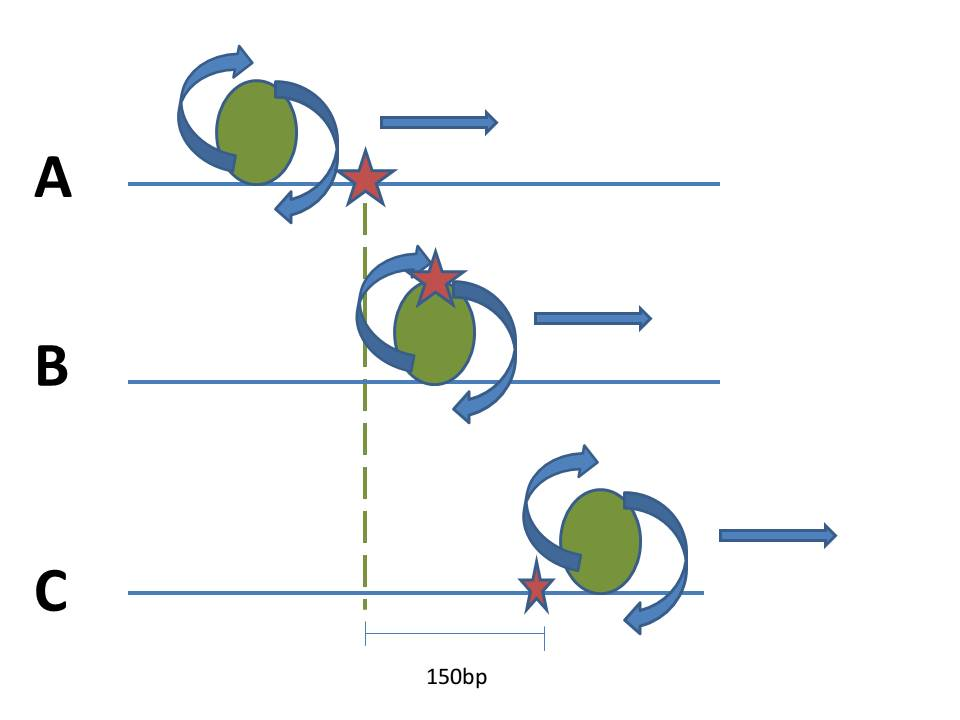
\includegraphics[width=0.7\linewidth]{Images/SlidingModel/histoneSlidingSingle}
				   	\caption{\tiny{\textbf{Three time points during a displacement of damage site (red star) caused by histone sliding. The displacement of the damage site is equivalent to the length of DNA wrapped on a histone. A displacement is measured in aerial distance from a reference point, and does not refer to an actual motion of the point on the DNA}}}
				   	\label{fig:histoneSlidingSingle}
				   \end{figure}
				   
				   \begin{figure}[H]
				   	\centering
				   	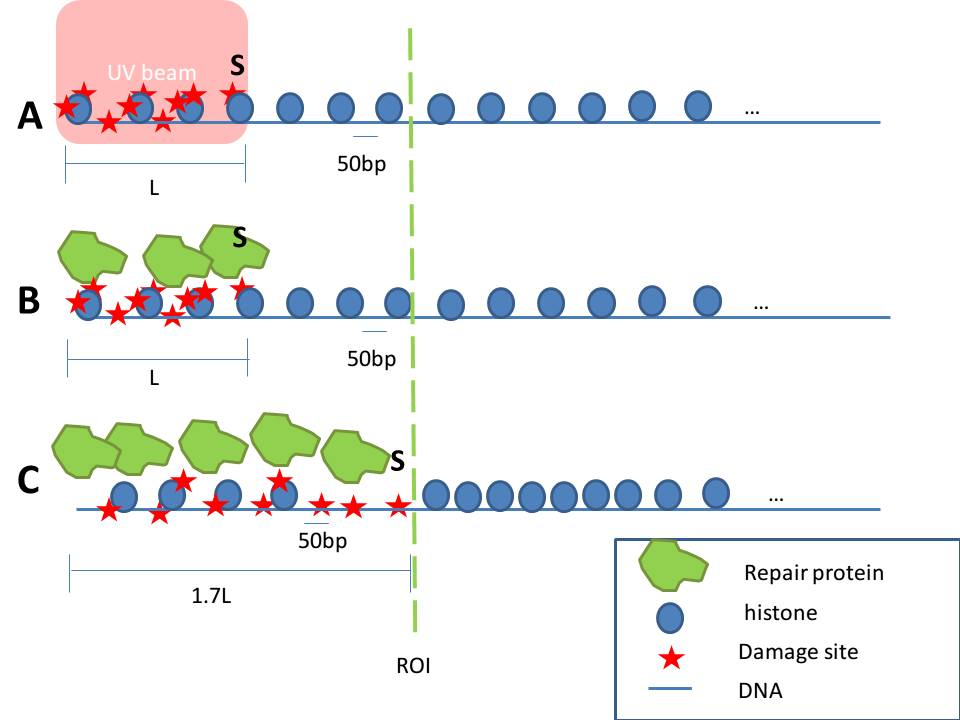
\includegraphics[width=0.7\linewidth]{Images/SlidingModel/histoneSlidingMulti}
				   	\caption{\tiny{\textbf{Expansion of the ROI due to nucleusome sliding. \textbf{A}. A UV beam (transparent red) damages DNA, with the point $S$ being the rightmost damage site \textbf{B}. Repair proteins (green polygons) are recruited to the damage site and expose the DNA in order the repair damages. \textbf{C}. Sliding the nucleosomes to the right in order to expose damage sites, translates the point $S$ from $S$ to $\beta$. Repair proteins follow the damage point to its new location. The presence of repair proteins in $\beta$ mark the ROI's boundary (vertical dashed green line). All DNA and histones to the right of $S$ are lost}}}
				   	\label{fig:histoneSlidingMulti}
				   \end{figure}
		
								
		\subsection{Expansion attributed to sliding and pushing sub-mechanisms}\label{subsection:ExpansionDueToSlidingAndPushing}
		The relative contribution of each sub-mechanism to the total expansion is estimated by dividing the expansion process into two: pushing and then pushing+sliding. The composition and order of events will be neglected in this description. 
		
	    If due to pushing up to a distance of $0<L<\beta$ we have lost a fraction of $k$ of both histones and DNA, we have for the total fraction of DNA and histone loss
         
		\begin{eqnarray*}
			d &=& k+\frac{\beta-L}{\beta}(1-k) \\
			h &=& k+\frac{(\beta-L)(\beta+\alpha)}{\beta l}(1-k)
		\end{eqnarray*}
		(see notation in previous subsection \ref{subsection:HistoneSlidingModel})		
     	
		The overall expansion radius to which sliding is responsible is thus 
		\begin{equation}\label{eq:expansionRadiusDueToSliding}
		L = \beta- \frac{\beta l(d-1)}{l(d-1) +\pi \beta(d-h)}
		\end{equation}
		
		Some values for the radius attributed to either mechanism are given in the figure below
		\begin{figure}[H]			
			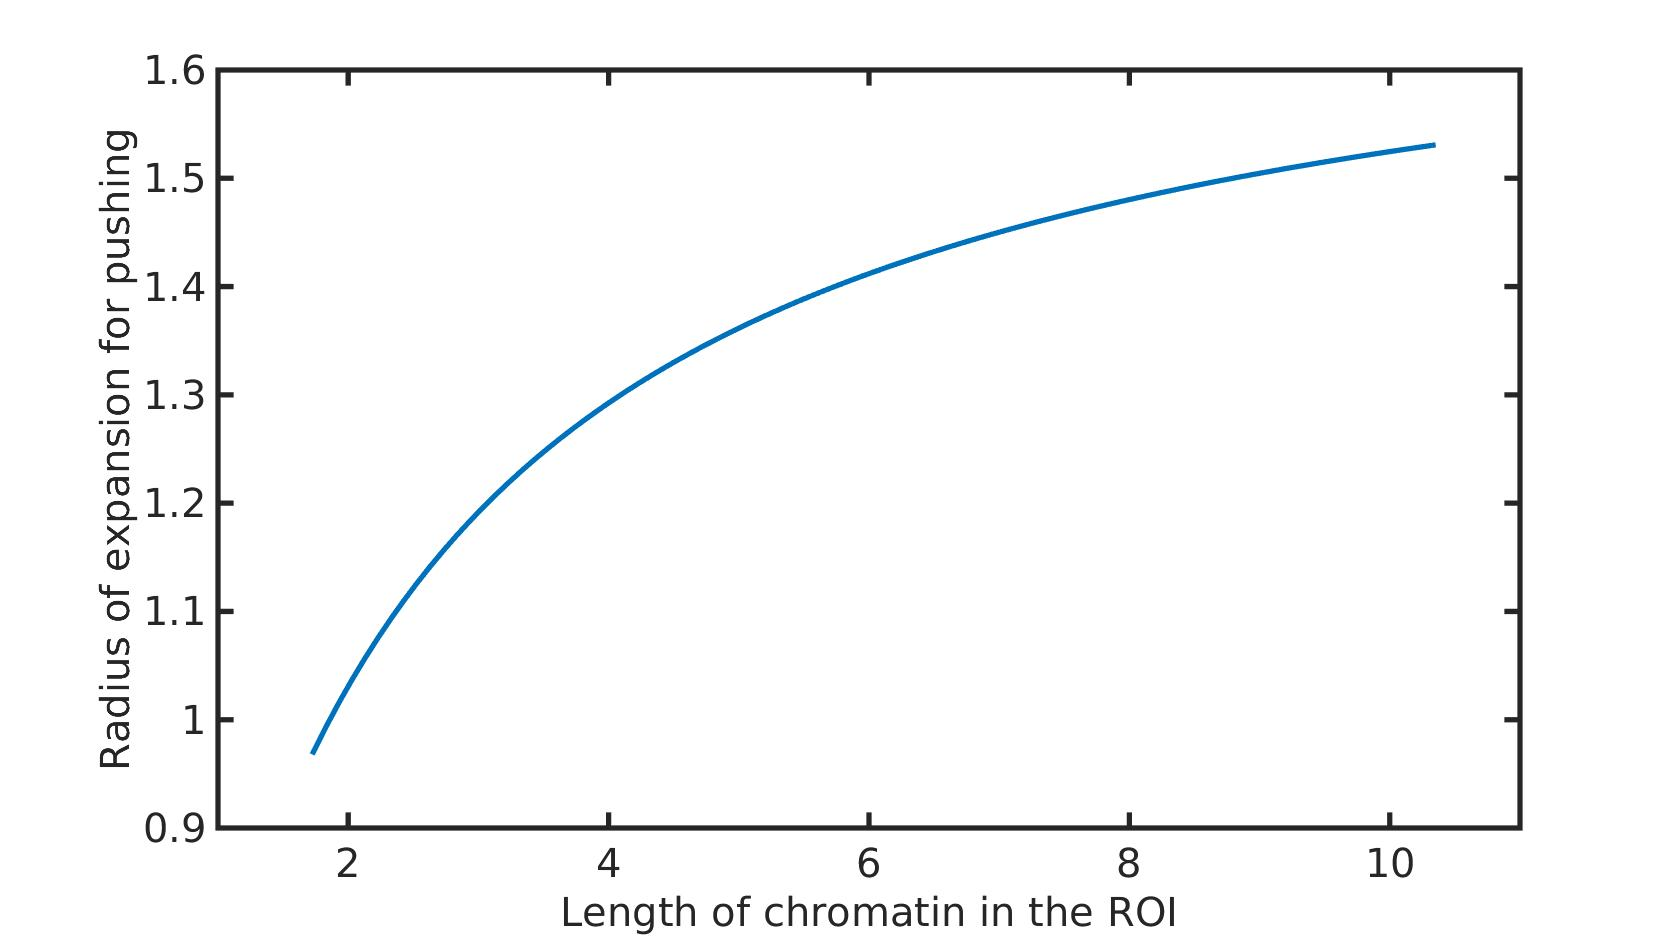
\includegraphics[width=0.5\linewidth, height=0.3\textheight]{Images/SlidingModel/radiusOfPushingVsLengthOfChromainInROI}
			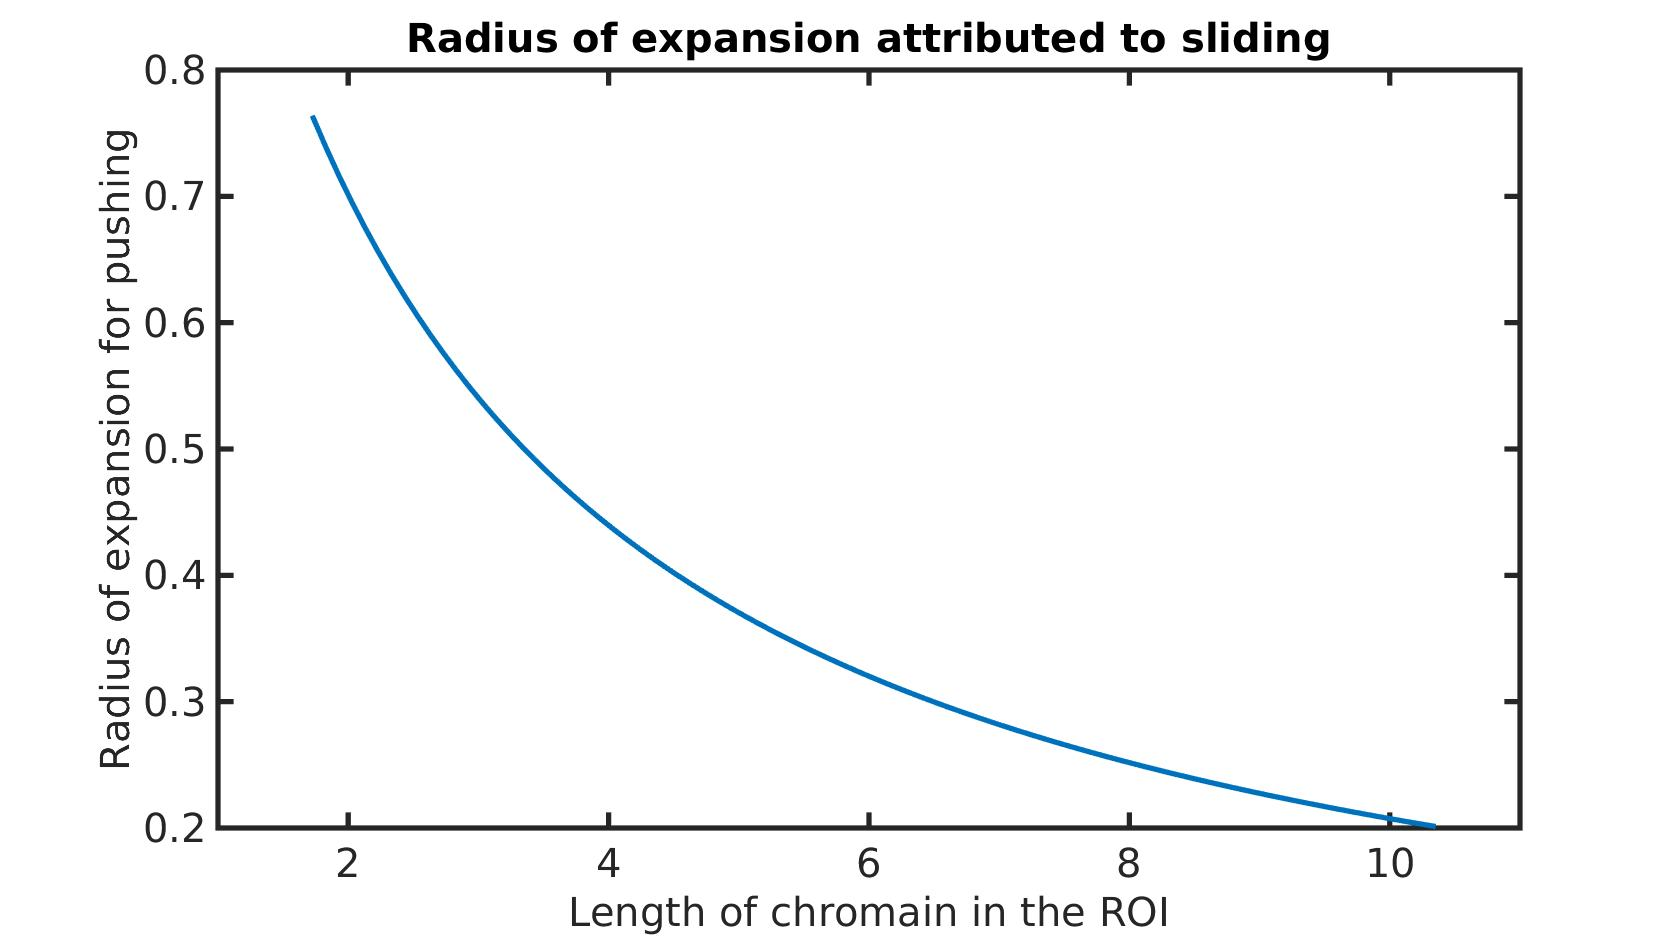
\includegraphics[width=0.5\linewidth, height=0.3\textheight]{Images/SlidingModel/radiusOfSlidingVsLengthOfChromatinInROI}
			\caption{\tiny{\textbf{The expansion radius attributed to pushing with no sliding (left) of chromatin as a function of the length of chromatin in the region, and it's complement, the radius of expansion attributed to pushing + sliding (right) as a function of the length of chromatin in the ROI. The ROI expansion is set to $\sqrt{3}$ and values of the chromatin length range from $\sqrt{3}$ to $7\sqrt{3}$}}}
			\label{fig:radiiVsLengthOfChromainInROI}
		\end{figure}
		
									
		\subsection{Estimation of the contribution of sliding to the expansion from the data}\label{subsection:estimationOfSlidingRadiusFromTheData}
		We have no direct access to the length of the chromatin expanded in the ROI. We estimate it indirectly from mass conservation considerations during expansion of the illuminated patch and Assuming uniform density of histones before UVC. 
		
		Measurement of the expansion of the patch shows 25-30\% increase in radius (Figure \ref{fig:patchExpansionMeasurement})
		\begin{figure}[H]
			\centering
			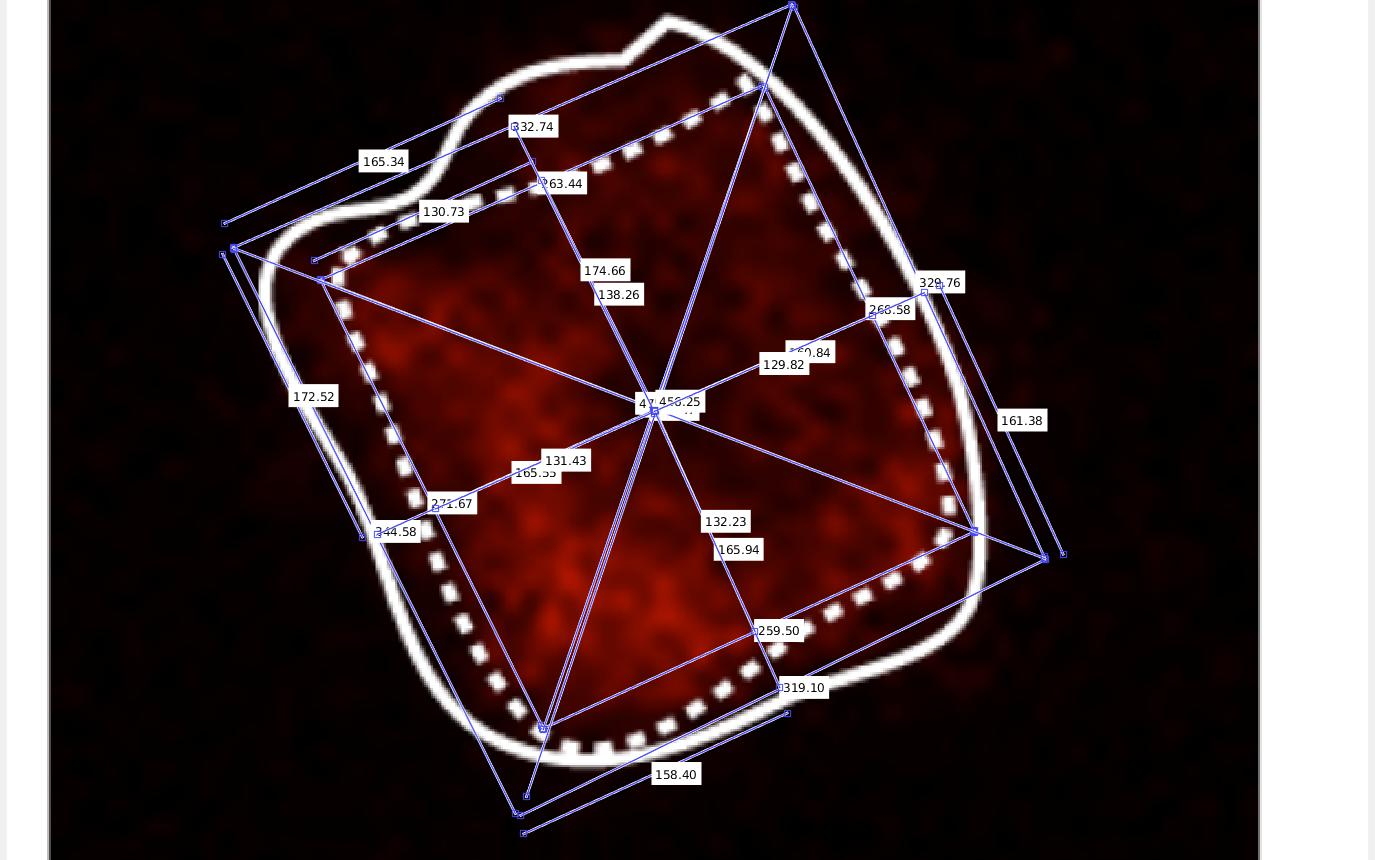
\includegraphics[width=0.5\linewidth, height=0.3\textheight]{Images/PatchExpansion/patchExpansionMeasurement}
			\caption{\tiny{\textbf{measurement of patch expansion from time 0  just before UVC (dashed) to 15 minutes post UVC (full line) the patch grows by 25-30\% of its initial radius, from 2.52 to the range [3.15,  3.28] }}}
			\label{fig:patchExpansionMeasurement}
		\end{figure}
		
		
		\begin{figure}[H]
			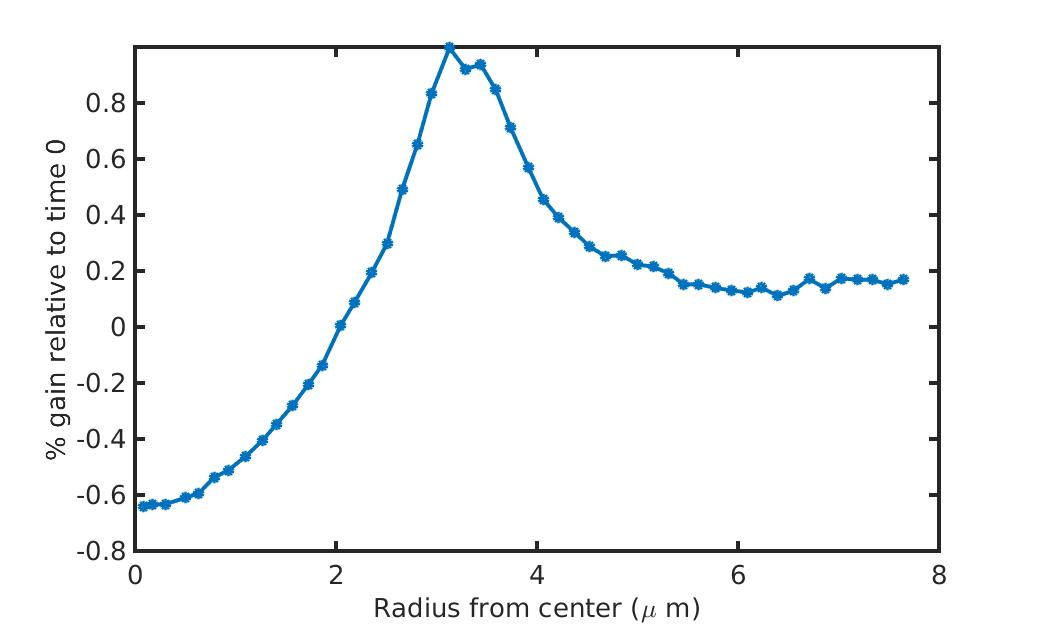
\includegraphics[width=0.5\linewidth, height=0.3\textheight]{Images/PatchExpansion/relativeGainNucleosomesConcentric}
			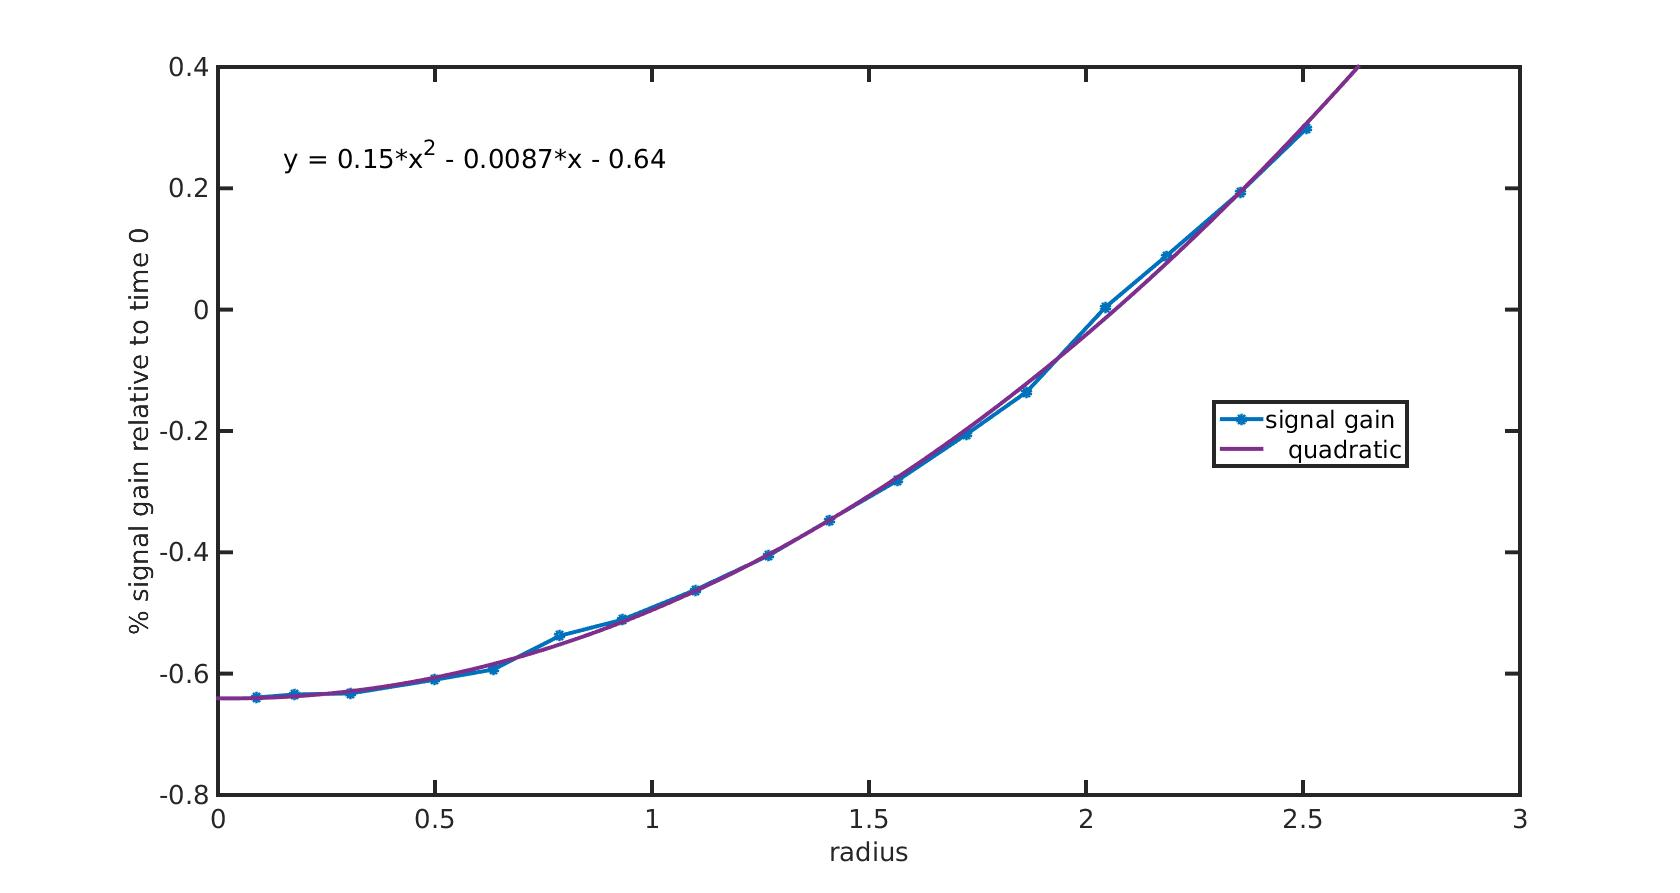
\includegraphics[width=0.5\linewidth, height=0.3\textheight]{Images/PatchExpansion/nucleosomeSignalGainConcentricFit}
			\caption{\tiny{\textbf{The relative gain 15 minutes post UVC relative to 0 minutes (left). A fit of the gain function up to the boundary of the patch (right) by a quadratic polynomial}}}
			\label{fig:relativeGainNucleosomesConcentric}
		\end{figure}
		
		Using 		
		\begin{equation}\label{eq:HistonePreservationConcentric}
		\frac{\int_0^RF(r)(y(r)+1)dr}{\int_0^RF(r)dr} =\gamma
		\end{equation} 
		with $F(r)$ the amount of histones in concentric ring between $r$ and $r+dr$, $y(r)$ the quadratic fit to the gain function, and $\gamma$ is the fraction of histones in a region of radius $R$. We find that the expansion radius attributed to sliding is in the range 0.34 to 0.46 $\mu m$.  
		
		Plugging this estimation in the formula for the $L$ gives us an estimation of the ratio between the ROI radius and the length of DNA stretched from the damage zone
		\begin{equation}\label{eq:ratioOfDNALengthToRoiRadius}
		\frac{l}{\beta} = \frac{L\pi(d-h)}{(\beta-L)(d-1)}
		\end{equation}				
		
		\subsection{Simulation of expansion and repair}\label{subsection:SimulationOfExpansionAndRepair}
		To examine the organization of the chromatin after repair, we perform 2D simulations of the damage process and expansion. Expansion of 1.7 is obtained for a Rouse polymer having 500 monomers, with 80\% additional cross-links. 		
		After UVC, cross-links from damaged monomers are removed. We simulate crowding around damage zones by employing an harmonic potential around damaged monomers having a radius of exclusion between 0.6-0.65.
		
		
				
	\begin{figure}[H]
	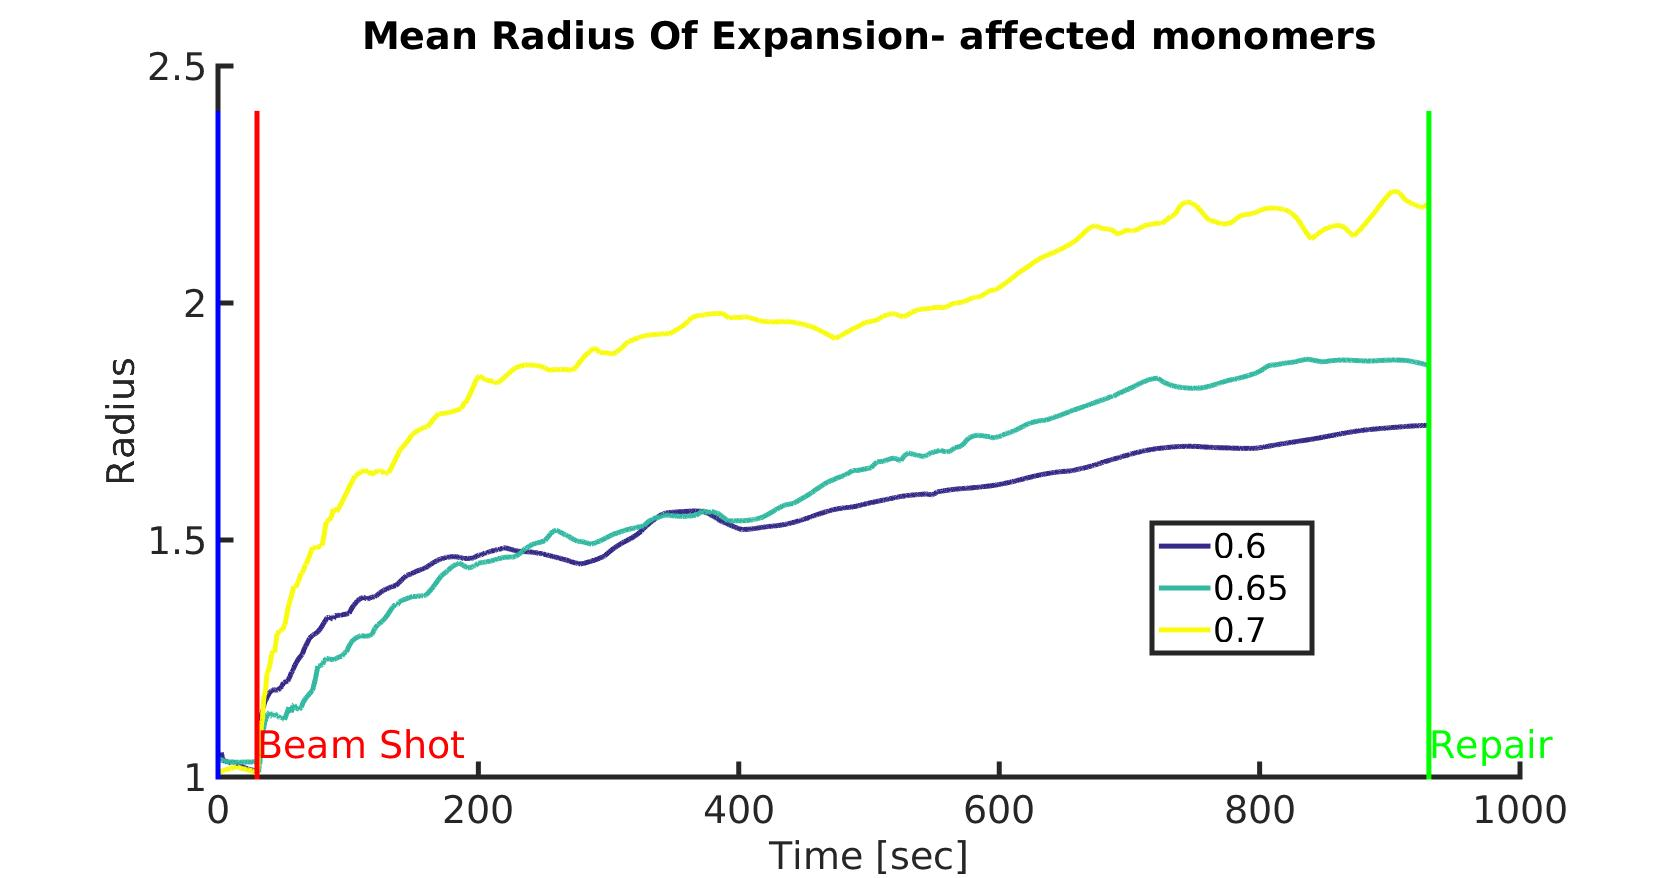
\includegraphics[width=0.5\linewidth, height=0.3\textheight]{Images/Simulations/meanRadiusOfExpansionAffected}
	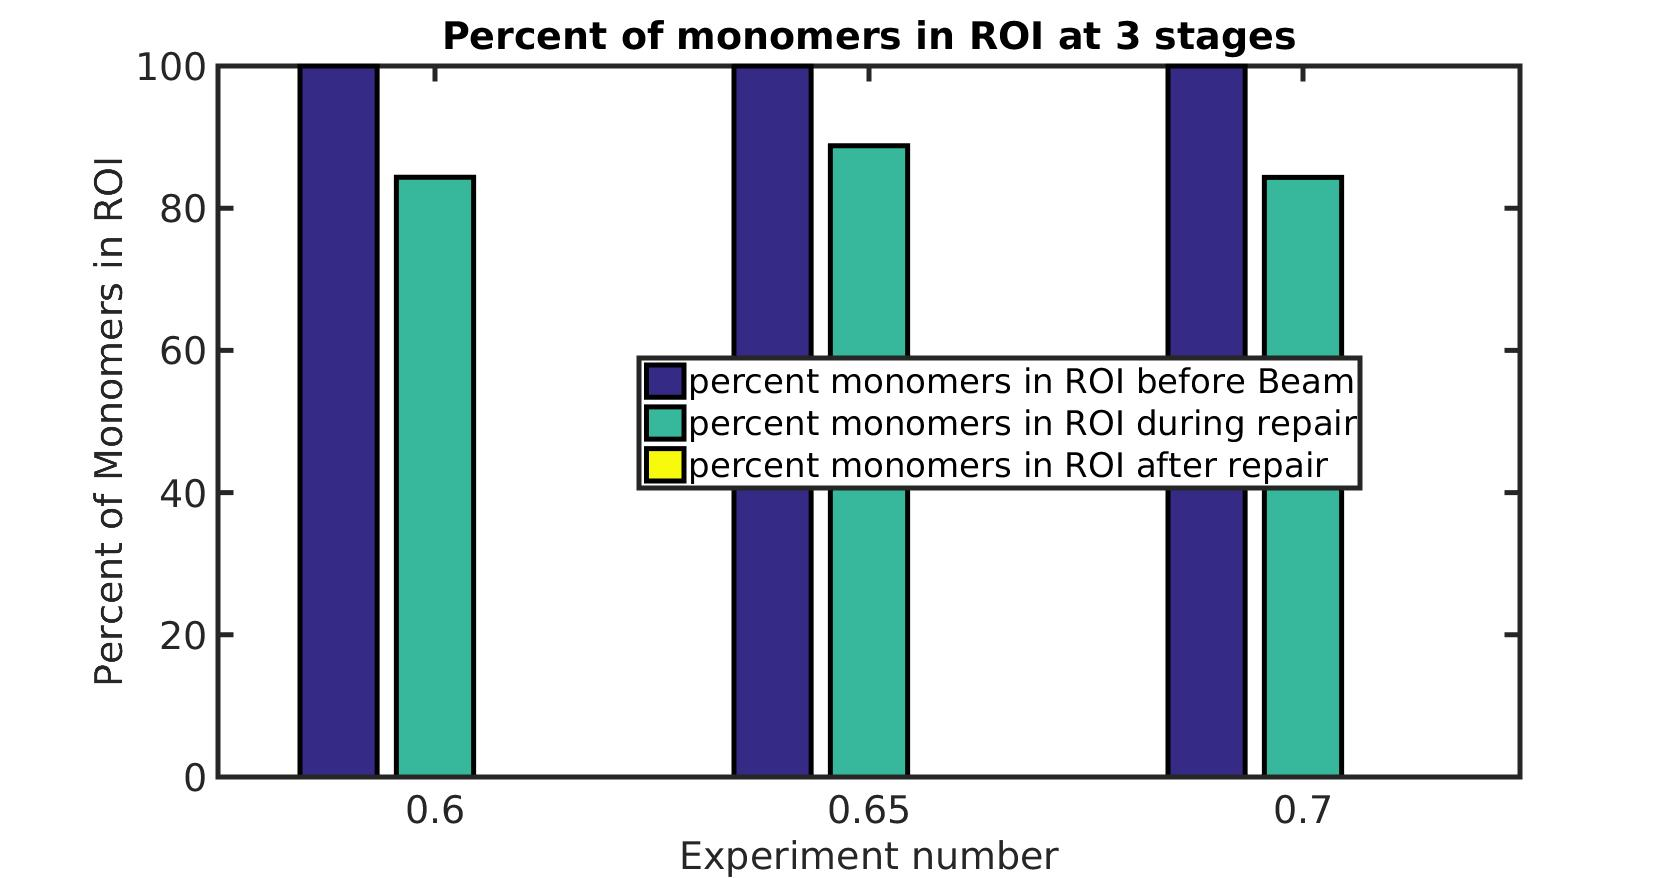
\includegraphics[width=0.5\linewidth, height=0.3\textheight]{Images/Simulations/percentOfMonomersInROI}
	\caption{}
	\label{fig:meanRadiusOfExpansionAffected}
	\end{figure}


\end{document}